% Created 2020-08-04 Tue 22:08
% Intended LaTeX compiler: pdflatex
\documentclass[a4paper]{article}
\usepackage[utf8]{inputenc}
\usepackage[T1]{fontenc}
\usepackage{graphicx}
\usepackage{grffile}
\usepackage{longtable}
\usepackage{wrapfig}
\usepackage{rotating}
\usepackage[normalem]{ulem}
\usepackage{amsmath}
\usepackage{textcomp}
\usepackage{amssymb}
\usepackage{capt-of}
\usepackage{hyperref}
\author{Tigany Zarrouk}
\date{\today}
\title{Multi-scale investigation of dislocation mediated carbon migration in iron}
\hypersetup{
 pdfauthor={Tigany Zarrouk},
 pdftitle={Multi-scale investigation of dislocation mediated carbon migration in iron},
 pdfkeywords={},
 pdfsubject={},
 pdfcreator={Emacs 26.3 (Org mode 9.1.9)}, 
 pdflang={English}}
\begin{document}

\maketitle
\tableofcontents

\begin{abstract}

We investigate the validity of a dislocation-assisted carbon migration
mechanism underpinning the formation of dark etching regions in
bearing steels undergoing high-cycle fatigue through use of a
multi-scale approach: from quantum mechanics,
to stochastic simulations. We start from tight binding simulations of
$1/3\langle 111 \rangle$ screw dislocations to obtain the 2-d Peierls
potential and Fe-C binding energies. These become ingredients for a line-tension
model of the $1/3\langle 111 \rangle$ screw dislocation to obtain the kink-pair formation
energy as a function of stress and carbon concentration. Finally,
3-d kinetic Monte-Carlo simulations of dislocations in an environment
of carbon are used to ascertain which temperature and stress regimes
dislocation-assisted carbon migration is a valid mechanism. 

\end{abstract}


\section{Introduction}
\label{sec:orged5d696}

\begin{itemize}
\item What is the DER?
\item How is it formed?
\item What does carbon binding to dislocations have to do with its formation?
\begin{itemize}
\item What mechanisms are at play?
\item Where is the crux of the argument?
\end{itemize}
\item How does/will atomistic modelling help?
\item What simulations do I do to figure this out?
\end{itemize}



Martensitic steels are frequently used in bearings due to their resilience to service conditions,
being subject to high rotational speeds and contact pressures. However, under cyclic loading
exceeding a given contact stress, the microstructure of the steel can decay due to the accumulation
of plasticity. This signals the onset of rolling cycle fatigue (RCF), which increases the risk of
failure from subsurface crack initiation. The microstructural decay corresponds to the observation
of Dark Etching Regions (DERs) as seen in optical microscopy, where the darkness of the images is due
to the higher reactivity of the phases which compose the DER region to the etchant; exacerbated by
the roughness of the DER region.


The degradation of the martensitic microstructure is due to a process of carbon migration driven
by plasticity-induced dislocation glide [CITATION]. The martensite is transformed to ferrite (microband
and elongated forms) through this process. Residual carbides, untouched at the start of DER
formation, gradually dissolve as a result of highly localized plasticity. RCF progression
leads to the formation of low and high angle ferrite features, composed from the microband and elongated
ferrite. Carbon atoms segregate from the martensitic matrix and (partially) dissolved
residual carbides, to form lenticular carbides between these ferrite bands. 

However, there is no consensus on where carbon migrates to with the onset of DER formation: where
does excess carbon from the martensitic matrix find itself, when the structure decays to low solubility (0.02\%)
ferrite. It is not known whether carbon atoms inside the martensite are transported towards the
transition carbides, a mechanism proposed by Fu \emph{et al.}
\cite{fu17_strain_induc_marten_decay_bearin,Fu2017}, or if they segregate to the boundaries of ferrite
microbands/elongated ferrite.

Probing the fundamental mechanisms behind DER formation experimentally have proven difficult and
inconclusive. A multi-scale modelling approach can shed light on the fundamental mechanisms behind
DER formation. Atomistics can provide information of the Peierls energy landscape of dislocations
in iron; and how this landscape is modified by the binding of carbon to dislocations. This data can be used in a
line tension model, to ascertain the kink-pair nucleation energies of dislocations as a function of carbon content and
stress. Finally, one can use a kinetic Monte Carlo model of dislocation kink-pair nucleation in an
environment of carbon to determine in what regimes of temperature, stress and carbon
concentration, dislocation-assisted carbon migration becomes a feasible mechanism behind DER
formation, and what happens to the dislocations how does carbon move in these
regimes. 

With this work as a foundation, one should be able to compare the affinity of carbon to
dislocations/grain boundaries: specifically carbides and grain boundaries, clarifying if carbides
grow, as in the theory by Fu, or if they dissolve, as some optical data suggests. 


Fu \emph{et al.} propose that most carbon is initially segregated to dislocations in martensite. Strain
generated by pulsating stresses allow dislocations to escape their carbon rich
environment. The dislocations, now free, re-attract carbon, allowing the Cottrell atmosphere to
reform, subsequently pinning the dislocations. This creates a net carbon flux, which according to
their theory, would segregate to carbides, increasing their size. However this is at odds with
theory: if carbides were to form in martensite, they should follow the Bagaryatskii/Isaichev
orientation relationship. Carbides formed within the DER region have an irregular shape, which
must be due to the incomplete \emph{dissolution} of residual carbides, which is at odds with the theory
of carbide growth. 


We propose that dislocations are crucial in all aspects of DER formation. Observation of DERs are
related to dislocation configurations at a particular number of stress cycles with the added
interactions of dissolved carbon. Tempered and residual carbides dissolve upon interaction with
dislocations. The carbon atoms that are trapped by the dislocations can cause pinning, affecting their
movement and rearrangement. Dislocation models are able to explain the hardening and softening
characteristics with application of contact pressure. With further knowledge of the fundamental
mechanism behind DER formation, we can surpress dislocation motion in the initial martensitic
matrix. 

As RCF continues, ferrite microbands decay to nanocrystalline ferrite. At the later stages of RCF,
there is a reduction in dislocation density within the grain boundaries of nanocrystalline
ferrite, which reduces the solubility of carbon, causing the formation of lenticular carbides
around the ferrite bands. 

Smelova proposes that the formation of ferrite phases are the
result of recrystallisation processes, which also bring doubt upon the work of Fu \emph{et
al.}.

\begin{itemize}
\item Maybe explain the reasoning behing Fu's conclusion
\item Why are other observations more reasonable?
\item Where do my simulations fit into this? 
\begin{itemize}
\item Segregation energies of carbon do dislocation to cause transport
\item This can lead to a comparison of segregation energies between ferrite boundaries and carbides
eventually (relative to carbon trapped in dislocations in bcc iron).
\end{itemize}
\end{itemize}




Due to the high dislocation density of martensite, all dissolved
carbon is segregated to dislocations---which also pin the
dislocations. With applied stress, the dislocations become unpinned
and mobile. Dislocations multiply/annihilate; with annihilation,
carbon becomes in ordinary solution, which is available to
diffuse. This diffusion causes the formation of ferritic
microbands. The process of annihilation needs to be understood. 

Hedman/Slycke propose that the degradation of the DER can by
described by the growth of carbides, where the carbide sized are
described by Ostwald ripening, and carbon diffuses both thermally
and mechanically by dislocation glide. 

Slycke proposes a creep deformation based mechanism which is
controlled by vacancies produced by the climb of dislocations. 


\subsection{Mechanisms}
\label{sec:org082d1e0}

There are many proposed mechanisms for DER formation.

Bush proposes that DER formation is governed by an
exchange of material between the carbides and the matrix, which is
evidenced by the formation of intrusions/extrusions within the
microstructure. 

Swahn proposes that the transformation mechanisms which lead to the
formation of new features in DER are due to the redistribution of
carbon present in the initial microstructure, which in solution in
the martensite, and due to the dissolution of carbides. 

They further detail that initially, stress induced carbon diffusion
leads to the diffusion of carbon from the martensitic lattice to
the various defects in the material (mainly dislocations). 
As plastic deformation accumulates, the movement of dislocations
creates carbon rich grain boundary-type interfaces. 

It is not certain what role and timescale the dissolution of
carbides occurs on. 

High operating temperatures are known to accelerate DER formation. 

In early stage DER formation, there is a high density of ferrite
microbands. Later, regions of homogeneous nanocrystalline ferrite
(heavily deformed ferrite) are formed in a cell-like structure.







\section{Computational Method}
\label{sec:orgeed92d8}

\begin{itemize}
\item Use tight-binding model of Paxton and Elsaetter \cite{Paxton2013}.
\item Generate dislocations using anisotropic elasticity theory.
\item Create clusters of dislocations in both easy and hard core
configurations.
\item Place carbon in octahedral sites around the core
\item Calculate corrections (ZPE etc)
\end{itemize}


\section{Results}
\label{sec:org9c3804c}



\subsection{Peierls Potential}
\label{sec:org5a63924}

To determine the Peierls potential, we followed the procedure detailed in Itakura
\cite{Itakura2012}. Quadrupolar arrays of dislocations were constructed by placing dislocations of
antiparallel \(1/2\langle 111\rangle\) Burgers vectors in an "S" arrangement \cite{Clouet2012} \ref{sarrangementclouet}, with
initial displacements determined by the anisotropic elasticity solutions. These displacements
were modified to be periodic, thereby removing artificial stacking faults which would appear
between periodic images after the introduction of the dipole. This was achieved by the subraction
of a linear error term from the superposition of displacement fields arising from the
dislocations in the simulation cell and its periodic images \cite{vasilybulatov2006}. To accomodate
for the internal stress upon introduction of the dislocation dipole into a simulation cell, an
elastic strain was imposed on the cell, resulting in an extra tilt component being added to the
cell vectors \cite{Clouet2012,vasilybulatov2006}. Simulation cells were constructed with different
initial core positions, which were sampled from the triangular region "EHS" (easy, hard and
split) core positions, as detailed in \ref{fig:peierlspot}. To fix the dislocation positions during
relaxation, the three atoms surrounding the easy core, for each dislocation, were fixed during
relaxation. 


\begin{center}
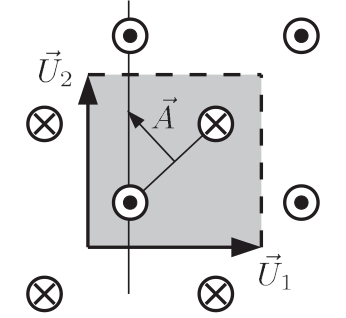
\includegraphics[width=.9\linewidth]{/home/tigany/Documents/docs/Management/Images/s_arrangement_clouet.png}
\label{org7bd8df3}
\end{center}


The interaction energy between the dislocation dipole and periodic images was defined differently
to that of Itakura's. We followed the prescription of Bulatov and Cai \cite{vasilybulatov2006} to
find a regularised interaction energy, which is independent of truncation limit, in contrast to
the formulas quoted in Itakura's papers \cite{Itakura2012}. In
isotropic elasticity, the elastic energy of a single dislocation dipole in an
infinite lattice is given by


\[ E_{\text{el}}^{\inf} = \frac{\mu b^2}{4\pi} ln( \frac{r}{r_{c}} )  \]

The contribution from periodic images to the correction is 

\[ E_{\text{img} } = E_{\text{el}} (\mathbf{a}, \mathbf{c}_i , r_c) - E_{\text{el}}^{\inf}
   (\mathbf{a}, r_c)\], 

where 

\[ E_{\text{img} = \sum_{\mathbf{R}}' E_{\text{dd}} (\mathbf{R}), \]

where \(\mathbf{R}\) is a sum over dislocation dipoles in the periodic images
exclusively. 

\[ E_{\text{dd}} (\mathbf{R}) = \frac{\mu b^2}{2\pi}
   \text{ln}\frac{|\mathbf{R}|^2}{|\mathbf{R}+\mathbf{a}|\cdot|\mathbf{R}-\mathbf{a}|}
   \]

"Ghost" dipoles are introduced to account for the conditional convergence
of the sum at \(\pm\alpha \mathbf{b}\) and \(\pm \beta\mathbf{b}\), where \(\alpha = \beta = 0.5\).  


The Peierls potential can be calculated by subtraction of the interaction energy of the
dislocations in the periodic array, from the energy of the easy core
configuration, which is the ground-state dislocation core configuration. 

\[ \Delta E_{\text{P}} = \Delta E^{\text{tbe}} - \Delta E_{\text{INT}} \]



        \begin{table}
    \begin{tabular}{c}
	     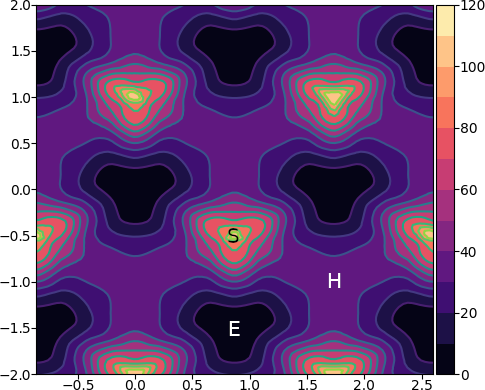
\includegraphics[width=0.8\textwidth]{../Images/itakura_dislocation_energy_landscape_2_labelled.png} \\
             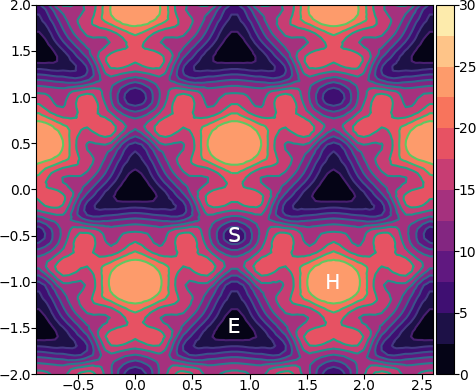
\includegraphics[width=0.8\textwidth]{../Images/tbe_dislocation_energy_landscape_pure_labelled.png}  \\
    \end{tabular}		
\caption{Comparison of 2d Peierls potentials of the $1/2\langle 111\rangle$ screw dislocation between DFT cite:Itakura2012 (top) and tight-binding (bottom). Data was interpolated using cubic splines. Energies are in $meV$, with x and y scales in units of $\sqrt{2} a_{\text{bcc}} = 2\sqrt{2/3}b$. "E", "H" and "S" correspond to easy, hard and split core positions respectively, with the latter also corresponting to atomic positions. The relative energies between the different core positions is smaller in tight-binding compared to DFT. The split core as seen in tight-binding is reminiscent of EAM potentials, where the split core energy is lower than that of the hard core. Some of this discrepancy can be attributed to the difference in simulation method: the cluster method may inhibit the relaxation of the core more than quadrupolar cells, due to finite size effects.}
	\label{fig:peierlspot}
    \end{table}



        \begin{table}
    \begin{tabular}{c}
	     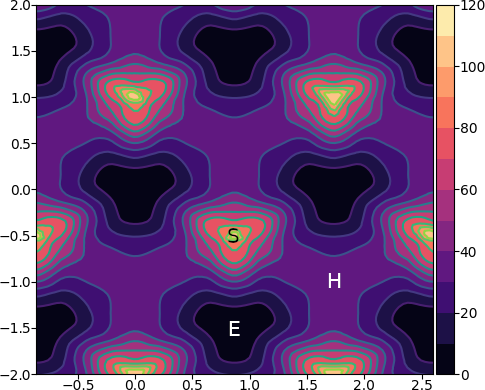
\includegraphics[width=0.8\textwidth]{../Images/itakura_dislocation_energy_landscape_2_labelled.png} \\
             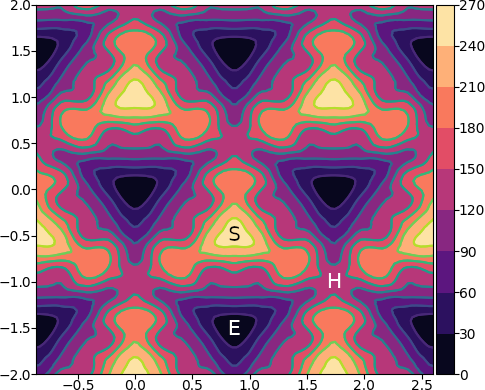
\includegraphics[width=0.8\textwidth]{../Images/tbe_dislocation_energy_landscape_2_labelled.png}  \\
    \end{tabular}		
\caption{Comparison of 2d Peierls potentials of the $1/2\langle 111\rangle$ screw dislocation between DFT cite:Itakura2012 (top) and tight-binding (bottom). Data was interpolated using cubic splines. Energies are in $meV$, with x and y scales in units of $\sqrt{2} a_{\text{bcc}} = 2\sqrt{2/3}b$. "E", "H" and "S" correspond to easy, hard and split core positions respectively, with the latter also corresponting to atomic positions. The relative energies between the different core positions is smaller in tight-binding compared to DFT. The split core as seen in tight-binding is reminiscent of EAM potentials, where the split core energy is lower than that of the hard core. Some of this discrepancy can be attributed to the difference in simulation method: the cluster method may inhibit the relaxation of the core more than quadrupolar cells, due to finite size effects.}
	\label{fig:peierlspot2}
    \end{table}


Comparison of 2d Peierls potentials of the \(1/2\langle 111 \rangle\) screw dislocation between
DFT can by found in \cite{Itakura2012}. Data was interpolated using 2d cubic splines. "E", "H"
and "S" correspond to easy, hard and split core positions respectively, with the latter also
corresponding to atomic positions. The relative energies between the different core
positions is smaller in tight-binding compared to DFT; most notably, the energies. This is
an artifact in the model, which has been validated in NEB calculations of the \(1/2\langle
	111\rangle\) screw dislocation Peierls barrier, as calculated with NEB, is roughly half that
when compared to DFT \textbf{ref Luke's Thesis}. The split core as seen in
tight-binding is reminiscent of EAM potentials, where the split core energy is lower than
that of the hard core, \emph{but first, to check that this is so, one must check that
the interaction energy between dislocations follows Bulatov and Cai}.

This may be attributed to lack of core electron	repulsion, resulting from the sd-iron tight-binding model. 

\begin{center}
\begin{tabular}{rrrrr}
Pos & \(\Delta E_{\text{INT}}\) & \(\Delta E_{\text{tbe}}\) & \(\Delta E_{\text{P}}\) & \(\Delta E_{\text{P}}^{\text{DFT}}\)\\
\hline
1 & 0 & 0 & 0 & 0\\
2 & -0.7 & 7.3 & 7.9 & 3.2\\
3 & -1.4 & 16.0 & 17.4 & 19.2\\
4 & -2.0 & 22.2 & 24.2 & 31.1\\
5 & -2.5 & 24.8 & 27.4 & 39.3\\
6 & -3.3 & 3.0 & 6.3 & 11.5\\
7 & -6.5 & 7.1 & 13.6 & 39.9\\
8 & -9.6 & 13.0 & 22.6 & 75.2\\
9 & -12.5 & 5.4 & 17.9 & 108.9\\
10 & -4.8 & 22.1 & 26.9 & 34.8\\
11 & -7.2 & 18.2 & 25.4 & 37.9\\
12 & -9.8 & 14.0 & 23.8 & 60.7\\
13 & -3.8 & 11.5 & 15.3 & 17.6\\
14 & -6.9 & 15.1 & 22.0 & 29.9\\
15 & -4.3 & 18.6 & 22.9 & 39.7\\
\end{tabular}
\end{center}

\subsection{Hard and easy core relaxations}
\label{sec:org5130498}

To determine the binding energy of carbon to dislocations, we used the
cluster method; where the simulation cells consist of a circular cluster of
atoms, split into two regions, with a single dislocation introduced into the
centre by using the anisotropic elasticity solutions. Each of the clusters
were centred on the easy or hard core positions. The cluster of atoms was
split into two regions: a central region of dynamic atoms with radius \(R_1\),
and an annulus of atoms, between \(R_1\) and \(R_2\), which were fixed to the anisotropic
elasticity solutions. 

Initially, large cells of with \(R_1 = 6\sqrt{2}a_{\text{bcc}}\), and \(R_2 =
   7\sqrt{2}a_{\text{bcc}}\) and depth of single burger's vector, were relaxed
for both the easy and hard cores, which consisted of 522 and 540 atoms
respectively. The three atoms surrounding the core were constrained, to only
relax in \(X-Y\) plane, to stop the core from moving upon relaxation. The
k-point sampling mesh for each of these cells was 1x1x24, with a charge
tolerance for self-consistency of \(1e-6\). Atoms were relaxed until the force
on each atom was less than \(1e-3\) eV/\AA{}.  

From the relaxed cells, a smaller region of 174 atoms, with \(R_1 =
   3\sqrt{2}a_{\text{bcc}}\), and \(R_2 = 4\sqrt{2}a_{\text{bcc}}\), was cut from
the dynamic regions. This smaller cell was extended to a thickness of 3\(b\) in
the \(Z\) direction. Carbon interstitials were inserted into octahedral sites
near the dislocation core, in the middle layer. Exploiting reflection and
rotational symmetry, allows us to use only 10 interstitial
sites to obtain the binding energies of carbon \(\sim2\) b from the core. 

The three atoms surrounding the core in the first and third layers were again
constrained to relax only in the \(X\) and \(Y\) directions. No such constraints
were imposed on the middle layer. 

The core energy difference can be estimated by the difference
between the excess energies of the easy and hard cores in the limit
that \(\text{ln}{\frac{R}{R_0}) \rightarrow 0\). At the smallest
value, one finds that the core energy difference \(\Delta
   E_c^{\text{Easy-Hard}} = 76\) meV/b. This is in agreement with the
results of Itakura \cite{Itakura2012}, of 82 meV/b.


As found in DFT simulations by Ventelon \cite{Ventelon2015}, when a carbon was placed in the
vicinity of a relaxed easy dislocation core---in either of the two nearest, distinguishable,
octahedral sites---a spontaneous reconstruction of the dislocation core occurred: from easy to
hard. Upon reconstruction, the dislocation core moved to a neighbouring triangle, when looking along the \(\langle
   111\rangle\) direction, where the carbon found itself situated in the centre.




Plot of dislocation energy as function of cluster size. 

\begin{center}
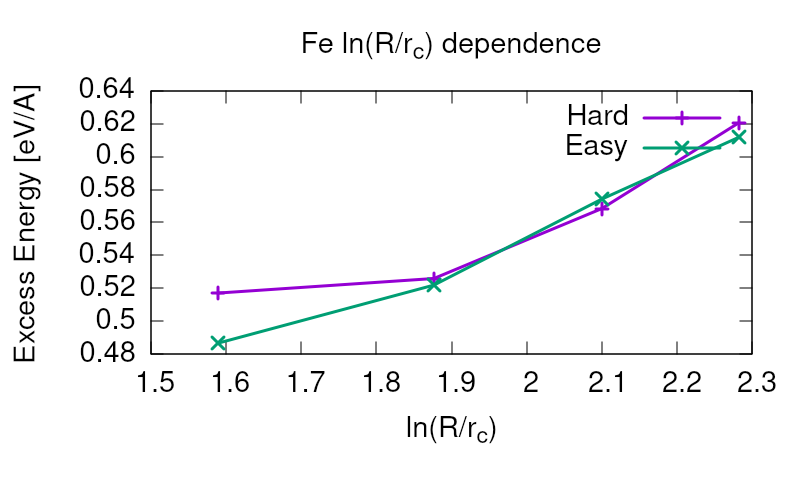
\includegraphics[width=.9\linewidth]{/home/tigany/Documents/docs/Management/Images/img_fe_size_dependence_on_log_of_core_radius.png}
\end{center}



\begin{table}	
    \begin{tabular}{c}
 	          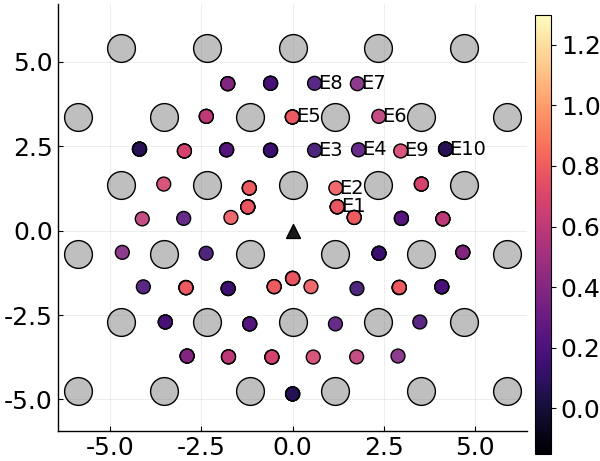
\includegraphics[width=0.85\textwidth]{../Images/easy_core_fe_C_positioning_energies_e10.png}  \\
 	          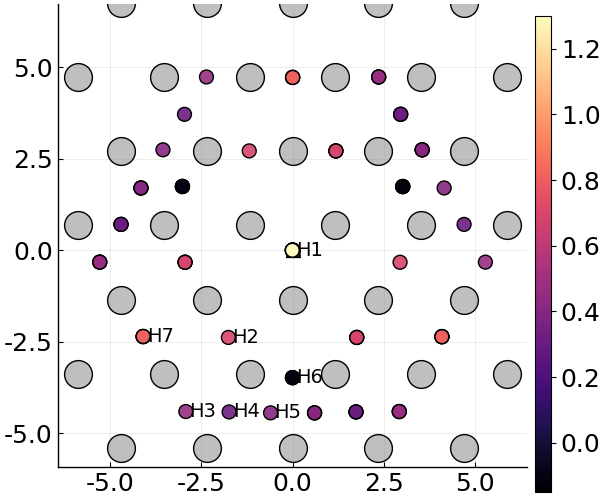
\includegraphics[width=0.85\textwidth]{../Images/hard_core_fe_C_positioning_energies_h7.png}  \\

     	     \end{tabular}		
\caption{ Final positions and binding energies (eV) of carbon around the easy core (top) and hard core (bottom). The core was constrained by fixing the top and bottom three atoms surrounding each of the cores. As shown by Ventelon cite:Ventelon2015, the first and second closest octahedral sites to the hard core have their minimum energy inside the hard core. }
   \end{table}


Following the paper by Itakura
\cite{itakura13_effec_hydrog_atoms_screw_disloc} we calculated the
binding energy of carbon each of the screw dislocation cores. 

The solution energy is given by 
\[ E_s = E_{\text{d + C}} - E_{\text{d}} - E_{\text{C ref.}}, \]
where \(E_{\text{d + C}}\) is the total energy of a relaxed cluster with a
carbon interstitial and a dislocation, \(E_{\text{d}}\) is the total
energy of a relaxed cluster with a dislocation and \(E_{\text{C
    oct.}}\) is the total energy of relaxed a cluster with a single carbon in
an octahedral site.

The zero-point energy is calculated as in Itakura. After relaxation of the
C-dislocation system, a 3x3 Hessian matrix is constructed by taking the
numerical derivative of forces observed on the carbon atom after
displacement by \(\pm 0.015 \AA\) in each of the \(X\), \(Y\) and \(Z\) directions.
The three atoms surrounding the core on the first and third layers were
again fixed in \(Z\) coordinate. The zero-point energy is
given by

\[ E_z = \frac{1}{2} \sum_{i=1}^3 \frac{h}{2\pi} \sqrt{ k_i /
    m_{\text{C}} },  \]
where \(k_i\) are the eigenvalues of the Hessian and \(m_\text{C}\) is
the mass of carbon. 

The ZPE corrected solution energy is given by 
\[ E^{\text{Z}}_{s} = E_s + \Delta E_z,  \]

where \(\Delta E_z = E_z - E_{z\text{C ref.}}\) and \(E_{z\text{C ref.}} = 202.5 meV\) is the zero-point energy of carbon
situated in an octahedral site in a perfect cluster of the same size. 


\begin{table*}
\label{orge77f861}
    \begin{tabular}{cccccc}
    \hline
Site Type & distance from core [b] & $E^{z}$ [eV] & $\Delta E^{z}$ [eV] & $E_b$ [eV] & $E_b^{z}$ [eV]  \\ 
     \hline
% 00        &                    --  &   0.203      &               0.000 &             &         --     \\
%           &                        &              &                     &             &                \\
E1        &                   0.57 &   0.185      & 	     -0.018 &       0.793 &          0.775 \\
E2        &                   0.70 &   0.202      & 	     -0.001 &       0.793 &          0.793 \\
E3        &                   0.99 &   0.205      & 	      0.002 &       0.137 &          0.139 \\
E4        &                   1.21 &   0.208      & 	      0.005 &       0.229 &          0.234 \\
E5        &                   1.36 &   0.210      & 	      0.008 &       0.784 &          0.791 \\
E6        &                   1.66 &   0.209      & 	      0.007 &       0.597 &          0.603 \\
E7        &                   1.89 &   0.206      & 	      0.003 &       0.385 &          0.388 \\
E8        &                   1.77 &   0.203      & 	      0.000 &       0.177 &          0.178 \\
E9        &                   1.52 &   0.201      & 	      0.000 &       0.683 &          0.683 \\
E10       &                   1.95 &   0.202      & 	      0.000 &       0.067 &          0.067 \\
H1        &                   0.00 &   0.196      & 	     -0.006 &       1.298 &          1.291 \\
H2        &                   1.19 &   0.210      & 	      0.007 &       0.691 &          0.698 \\
H3        &                   2.12 &   0.209      & 	      0.007 &       0.461 &          0.467 \\
H4        &                   1.91 &   0.207      & 	      0.005 &       0.311 &          0.316 \\
H5        &                   1.80 &   0.208      & 	      0.006 &       0.403 &          0.409 \\
H6        &                   1.40 &   0.207      & 	      0.005 &      -0.119 &         -0.114 \\
H7        &                   1.35 &   0.206      & 	      0.006 &       0.825 &          0.819 \\

    \end{tabular}		
    \caption{Table of energies leading to the zero-point energy corrected binding energy. }
\end{table*}

These binding energies agree well with experiment and previous
calculations. The maximum binding energy found by the Fe-C EAM
potential by Becquart \cite{Becquart2007}, was 0.41eV. Kamber
\emph{et al.} found a maximum binding energy of 0.5 eV. Cochardt
found a value of 0.71 eV, which is within 0.1eV of the largest
binding energy for the easy core. 

EAM calculations by Clouet \cite{Clouet2008} found a binding energy of ---- by calculating the
elastic dipole tensor within Eshelby theory. 
Hanlumyuang \emph{et al.} \cite{Hanlumyuang2010} conducted DFT calculations for the interaction energy 12\AA{} from the core,
and their calculations agreed with the continuum limit of Eshelby theory with ----. 


In work by Ventelon \cite{Ventelon2015}, the interaction energy of a carbon in a hard
core prism configuration was found to be 0.79eV for a thickness in the \(Z\) direction of 3\(b\) (0.73eV for \(6b\))---in the
convention that a positive binding energy indicates attraction. This is significantly lower than
the 1.29eV interaction energy of tight-binding. This discrepancy can be
partially explained due to the short cutoff of the carbon interactions in tight-binding---at
\(\sim a_{\text{bcc}} = 2.87 \AA\). In addition, these cells are not fully relaxed, as the three
atoms around the core are fixed in Z. As the carbon is separated from its periodic image by \(3b =
    8.61\AA\), there is no contribution from the repulsive C-C interaction from periodic images,
which is included within DFT.


In the mean-field model of Ventelon, we have
\[ E_{\text{int}}( c_d ) = E^{(0)}_{\text{int}} + \frac{\Delta E_{\text{Easy-Hard}}}{c_d} + c_d V_{\text{CC}} , \]

where \(V_{\text{CC}}\) is the C-C interaction energy which can be found by the equation. In
tight-binding \(V_{\text{CC}}= 0\), 



Distance dependence of binding energies. 

\begin{center}
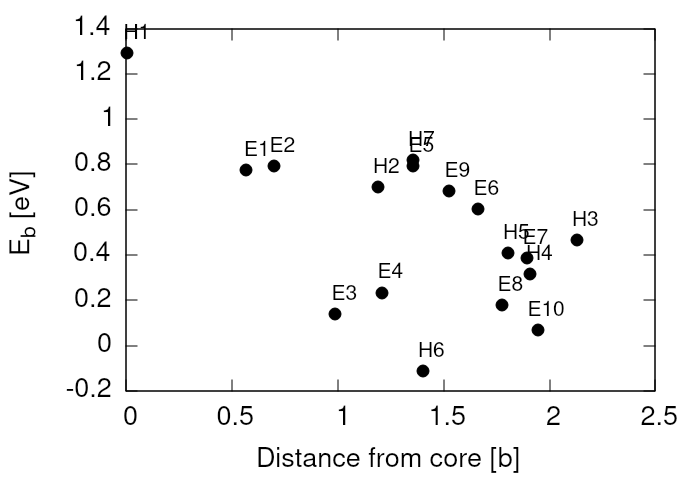
\includegraphics[width=.9\linewidth]{/home/tigany/Documents/docs/Management/Images/fe_c_binding_energy_distance.png}
\end{center}



\subsection{Line Tension}
\label{sec:orgbf9bc46}


One is still doing the work for the line tension model. This model views the dislocation
as an elastic string which moves on the Peierls potential \(\Delta E_{\text{P}}\). One is
using the julia implementation of the NEB algorithm by Ortner \cite{Makri2019}.
The equilibrium line shape \(y(x)\) of the dislocation is the solution to the 1D Klein-Gordon
type equation \cite{Rodney2009}:

\[ - \frac{\text{d} ( \Delta E_{\text{P}}[y(x)] )}{\text{d} y(x) } + \sigma_{\text{A}} b + T \frac{\partial^2 y}{\partial x^2} = 0,\]

where, 

\[ T = E_L + \frac{\text{d}^2 E_L}{\text{d}\phi^2},  \]


\[ E_L = E_{\text{el}} + E_{\text{core}} = \frac{\mu b^2}{2\pi} \text{ln} \big
   ( \frac{R}{r_c}\big ) + E_{\text{core}}.\]


I have calculated the coefficients necessary for the line tension model. But there seem
to be differences between what Itakura states in his paper and the coefficients that are
measured in the Proville paper \cite{Rodney2009}. 

One thing I can do to check the coefficients are correct, is to fit to the the kink
shape from Luke's thesis to obtain the correct value for the line-tension \(T\).

\section{Discussion}
\label{sec:org0170a9d}


\begin{itemize}
\item How do the results of this work feed into C migration with
dislocations?
\item How valid is the theory we have vs Fu \emph{et al}.
\item 
\end{itemize}

\section{Future work}
\label{sec:org0599ccf}

\begin{itemize}
\item Validation of line-tension model by reproduction of the dislocation line shape from
Itakura 2012 \cite{Itakura2012}.
\item Compare tbe dislocation line shape with Itakura, and find the migration path of the dislocation from tbe data.
\item\relax [Optional] Create Ising model for easy and hard core an compare the binding energies like \cite{Lthi2019}.
\item\relax [Optional] Find the elastic dipole tensor to check the binding energy of C within anisotropic elasticity.
\item Choose the sites for which one can fit a function (lorentzian) for the interaction energy between C and Fe.
\item Find the kink-pair formation enthalpy, with and without carbon, to feed into the kMC
code.
\end{itemize}



\section{Conclusion}
\label{sec:org39b914c}


\begin{itemize}
\item Outline of the literature review 
\begin{enumerate}
\item Origin of DER formation through high-cycle fatigue
\item What is the DER region and what phases is it composed of?
\item What are the current mechanisms which explain this?
\begin{enumerate}
\item Why are they insufficient?
\end{enumerate}
\item Ouline of the work considering Fe-C dislocation modelling
\end{enumerate}
\end{itemize}

\section{Appendix}
\label{sec:org431338b}


\section{Bibliography}
\label{sec:org28669cd}
\label{orgb5f3c42}

\bibliographystyle{unsrt}

\bibliography{../bibliography/org-refs}
\end{document}